\documentclass{article}
\usepackage{amsmath}
\usepackage{amsfonts}
\usepackage{graphicx} % Required for inserting images
\graphicspath{ {./images/} }
\usepackage{mathtools}

\mathtoolsset{showonlyrefs}

\title{FYP}
\author{Johns Noble}
\date{January 2025}

\begin{document}

\maketitle

\newpage
\tableofcontents
\newpage

\section{Introduction}
\subsection{Cauchy Transform}
\begin{equation} \label{cauchy transform}
C_\Gamma f(z):=\frac{1}{2\pi i}\int_\Gamma \frac{f(t)}{t-z}dt
\end{equation}
This is analytic for $z \not\in \Gamma$. Define Hilbert Transform to be the limits from the right and the left.
\subsection{Orthogonal Polynomials}
\begin{center}
\begin{tabular}{ |c|c|c|c| } 
 \hline
	Family & Notation & Interval & $w(x)$ \\ 
 \hline
	Legendre & $P_n(x)$ & [-1,1] & $1$ \\ 
	Chebyshev (1st) & $T_n(x)$ & [-1,1] & $(1-x^2)^{-1/2}$ \\ 
	Chebyshev (2nd) & $U_n(x)$ & [-1,1] & $(1-x^2)^{1/2}$ \\
	Ultraspherical & $C_n^{(\lambda)}(x),\:\lambda>-\frac{1}{2}$ & [-1,1] & $(1-x^2)^{\lambda-1/2}$ \\
	Jacobi & $P_n^{(\alpha,\beta)}(x),\:\alpha,\beta>-1$ & [-1,1] & $(1-x)^\alpha(1-x)^\beta$ \\
 \hline
\end{tabular}
\end{center}
\section{Log and Stieltjes Transform}
In this section we will consider approaches to compute these weakly singular integrals
$$ \int_Alog||z-t||f(t)dt \qquad \int_A\mathbf{\nabla}log||z-t||f(t)dt $$
\begin{equation}\label{stieltjes transform}
	\mathcal{S}_Af(z):= \int_A\frac{f(t)}{z-t}dt \\
\end{equation}
\begin{equation}\label{log transform}
	\mathcal{L}_Af(z):= \int_Alog(z-t)f(t)dt
\end{equation}
Depending on the type of area which $A$ is we can begin by approximating $f$ using orthogonal polynomials.
\subsection{Transforms across Intervals}
We will try to formulate recurrence relations for these transforms across interval [-1, 1].
We are looking for looking for $\mathcal{S}_{[-1,1]}f(z)$.
Decomposing $f(z) \approx \Sigma_k f_kP_k(z)$ and writing $S_k(z):=\mathcal{S}_{[-1,1]}P_k(z)$ lets us write:
$$\mathcal{S}_{[-1,1]}f(z) \approx \Sigma_k f_kS_k(z)$$
This motivates finding fast methods to compute $S_k(z)$. Log kernels are approached similarly letting $L_k(z):=\mathcal{L}_{[-1,1]}P_k(z)$ and looking for recurrence relations.
\subsubsection*{Stieltjes}
Recall recurrence relation of Legendre Polynomials:
\begin{equation}\label{legendre recurrence}
	xP_k(x) = \frac{k}{2k+1}P_{k-1}(x) + \frac{k+1}{2k+1}P_{k+1}(x)
\end{equation}
Formulate three-term recurrence for their Stieltjes transforms.
\begin{equation}
\begin{split}
	zS_k(z) &= \int_{-1}^{1}\frac{zP_k(t)}{z-t}dt \\
	&= \int_{-1}^{1}\frac{z-t}{z-t}P_k(t)dt+\int_{-1}^{1}\frac{tP_k(t)}{z-t}dt \\
	&= \int_{-1}^{1}P_k(t)dt+\frac{k}{2k+1}\int_{-1}^{1}\frac{P_{k-1}(t)}{z-t}dt+\frac{k+1}{2k+1}\int_{-1}^{1}\frac{P_{k+1}(t)}{z-t}dt \\
	&= 2\delta_{k0}+\frac{k}{2k+1}S_{k-1}(z)+\frac{k+1}{2k+1}S_{k+1}(z) \\
	S_0(z) &= \int_{-1}^{1}\frac{dt}{z-t} = log(z+1)-log(z-1)
\end{split}
\end{equation}
We can extend this to work over a square using the recurrence over intervals:
\begin{equation}
\begin{split}
zS_{k,j}(z) &= z\int_{-1}^1\int_{-1}^1\frac{P_k(s)P_j(t)}{z-(s+it)}dsdt \\
&= \int_{-1}^1zP_j(t)\int_{-1}^1\frac{P_k(s)}{z-it-s}dsdt \\
&= \int_{-1}^1(z-it)P_j(t)S_k(z-it)+itP_j(t)S_k(z-it)dsdt \\
&= \int_{-1}^1P_j(t)(\frac{k}{2k+1}S_{k-1}(z-it)+\frac{k+1}{2k+1}S_{k+1}(z-it)+2\delta_{k0}) \\
&+i(\frac{j}{2j+1}P_{j-1}(t)+\frac{j+1}{2j+1}P_{j+1}(t))S_k(z-it)dsdt \\
&= \frac{k}{2k+1}S_{k-1,j}(z)+\frac{k+1}{2k+1}S_{k+1,j} \\
&+i\frac{j}{2j+1}S_{k,j-1}(z)+i\frac{j+1}{2j+1}S_{k,j+1}+4\delta_{j0}\delta{k0}
\end{split}
\end{equation}
\subsubsection*{Log}
We can begin by connecting log kernel to the Stieltjes kernel. To do this we define:$$S_k^{(\lambda)}(z):=\int_{-1}^{1}\frac{C_k^{(\lambda)}(t)}{z-t}dt$$
We let $F(x) = \int_{-1}^1f(s)ds$ and apply integration by parts on log transform:
\begin{equation}
\begin{split}
	\int_{-1}^1f(t)log(z-t)dt &= [-F(t)log(z-t)]_{-1}^1-\int_{-1}^1\frac{F(t)}{z-t}dt \\
	&= log(z+1)\int_{-1}^1f(t)dt-\int_{-1}^1\frac{F(t)}{z-t}dt
\end{split}
\end{equation}

\section{Polynomial Transforms}
We can begin to consider taking these transforms across different geometries.
Currently we have a way to find these transforms across [-1,1] but we will be trying to use this to solve other geometries.
The first type of geometry we should consider is one where we apply a degree $d$ polynomial transform to the interval:
$$p:[-1,1]\rightarrow \Gamma$$
We will show why the solution to a cauchy transform across this interval is as follows:
\begin{equation}
C_\Gamma f(z) = \Sigma_{j=0}^dC_{[-1,1]}[f\circ p](p_j^{-1}(z))
\end{equation}
Where $p_j^{-1}(z)$ are the $d$ pre-images of $p$.
In order to solve this we will use plemelj.
There are 3 properties that need to hold for a function $\psi: \Gamma \rightarrow \mathbb{C}$ to be a cauchy transform:
\begin{equation}\label{cauchy_conditions}\begin{gathered}
\underset{z\to\infty}{lim}= 0 \\
\psi^+(z)-\psi^-(z)= f(z) \\
\psi\;analytic\;on\;\Gamma 
\end{gathered}\end{equation}

Checking \eqref{cauchy_conditions}.1 we get that $\underset{z\to\infty}{p_j^{-1}(z)} = \infty \implies$
\begin{equation}\begin{split}
\underset{z\to\infty}{lim}C_\Gamma f(z) &= \Sigma_{j=1}^d \underset{z\to\infty}{lim}C_{[-1,1]}(f\circ p)(p_j^{-1}(z)) \\
&= \Sigma_{j=1}^d C_{[-1,1]}(f\circ p)(\underset{z\to\infty}{lim} p_j^{-1}(z)) \\
&= \Sigma_{j=1}^d 0 = 0
\end{split}\end{equation}

Checking \eqref{cauchy_conditions}.2 we need an expression for $\psi^+$ and $\psi^-$.
Let us begin by saying that we are looking for cauchy transform of point $s$ which happens to lie on $\Gamma$.
This means that there is a unique root of $t_k := p_k^{-1}(s) \in [-1,1]$.
TODO: Show that $\underset{z\to s^+}{lim} p_k^{-1}(s) =\underset{z\to p^{-1}(s)^+}{lim}$.
Taking limits of $\psi^+, \psi^-$ gives us:
\begin{equation}\begin{split}
\psi^+(s)&=\underset{z\to s}{lim}\:C_{[-1,1]}(f\circ p)(p_k^{-1}(z)) \\
&+\Sigma_{j\neq k}C_{[-1,1]}(f\circ p)(p_j^{-1}(s)) \\
&=C^+_{[-1,1]}(f\circ p)(p_k^{-1}(z)) \\
&+\Sigma_{j\neq k}C_{[-1,1]}(f\circ p)(p_j^{-1}(s)) \\
\end{split}\end{equation}
We can do a similar thing with $\psi^-$ and putting everything together:
\begin{equation}\begin{split}
\psi^+(s)-\psi^-(s)&=C_{[-1,1]}^+(f\circ p)(p_k^{-1}(s))-C_{[-1,1]}^-(f\circ p)(p_k^{-1}(s)) \\
&= (f\circ p)(p_k^{-1}(s)) = f(s)
\end{split}\end{equation}
In the case where $z \notin \psi, \psi^+=\psi^-$ which is expected since the area in between is analytic

TODO show that condition \eqref{cauchy_conditions}.3 holds
\section{Affine Transformations}
Affine transformations can be solved in 2 distinct ways:
We will begin by considering the case of solving for a horizontally skewed square with the following transformation:
$$\begin{pmatrix}x\\y\end{pmatrix}\rightarrow
\begin{pmatrix}\alpha x+\beta y\\y\end{pmatrix}$$
It can be shown that any affine transformation in the form of $(x, y)^T \rightarrow A(x,y)^T$ can be done by taking the above translation and performing scaling and rotations.
TODO: Show that this is indeed the case

\section{Quad Transform}
We can attempt to generalise the method of stieltjes on a square to work for any given quadrilateral. We can use the parameterisation: $$Q\begin{pmatrix}x\\y\end{pmatrix}\rightarrow
\begin{pmatrix}(1+x)(\alpha+\beta y)\\y\end{pmatrix}$$
Since our $\alpha, \beta > 0$, our $Q$ is invertible:
$$Q^{-1}\begin{pmatrix}s\\t\end{pmatrix}\rightarrow\begin{pmatrix}\frac{s}{\alpha+\beta t}-1\\t\end{pmatrix}$$

There are two approaches which were considered which vary in which functions we are using for our bases.
The first approach that was attempted would be to take the function approximation as follows:
$$f(x,y)=\Sigma_{k,j}c_{k,j}P_k(x)P_j(y), c_{k,j}\in \mathbb{R}$$
This method is simpler but it can be seen that we would have to be evaluating integrals of orthogonal polynomials outside the
$[-1,1]$ domain in which they are well behaved.
This would result in instable results

It is possible to think of the function space here as the bases of functions which we can add together to approximate the function.
In the approach above we can represent the bases to be $\{b_{kj}\}_{kj}$ where $b_{kj}(\textbf{x})=P_k(x)P_j(y)$
The approach we will focus on here is the approximation following taking an approximation using the function bases as follows:
\begin{align}
    f\circ Q(x,y) &= \Sigma_{k,j}c_{k,j}P_k(x)P_j(y),\:c_{k,j}\in \mathbb{R}\\
    f\circ Q(\textbf{x})&=\Sigma_{k,j}c_{k,j}b_{kj}(\textbf{x})\\
    Q\:invertible \implies
    f(\textbf{x})&=\Sigma_{k,j}c_{k,j}b_{kj}(Q^{-1}(\textbf{x}))
\end{align}
This means we have an altered set of basis based on $\alpha,\beta$ where the new basis can be represented as:
$$\{\tilde{b}_{kj}=b_{kj}\circ Q^{-1}\}_{kj}$$
In this approach we are need to be able to compute $$s_{kj}:=\int_{-1}^1 (\alpha+\beta t) \int_{-1}^1 \frac{P_j(t)P_k(s)}
{z-it-(\alpha+\beta t)(1+s)} ds dt$$
As you can see here there is a term in the denominator which is difficult to deal with as it is harder to seperate the $s$ and $t$ terms.
In order to begin we come up with a few different rearrangements of this equation:
\begin{align}
\tilde{s_{kj}} :&= \int_{-1}^1 \int_{-1}^1 \frac{P_j(t)P_k(s)}
{z-it-(\alpha+\beta t)(1+s)} ds dt\\
&= \int_{-1}^1\frac{1}{\alpha+\beta t}\int_{-1}^1 \frac{P_j(t)P_k(s)}
{\frac{z-it}{\alpha+\beta t}-1-s}dsdt\\
&=: \int_{-1}^1\frac{P_j(t)}{\alpha+\beta t}\int_{-1}^1 \frac{P_k(s)}{\tilde{z_t}-s} \\
\tilde{s_{kj}} &= \int_{-1}^1\int_{-1}^1
\frac{P_j(t)P_k(s)}{z-\alpha(1+s)-(i+\beta(1+s))t}dsdt \\
&= \int_{-1}^1\frac{P_k(s)}{\beta(1+s)+i}\int_{-1}^1 \frac{P_j(t)}{
	\frac{z-\alpha(1+s)}{\beta(1+s)+i}-t}dtds\\
&= \int_{-1}^1\frac{P_k(s)}{\beta(1+s)+i}\int_{-1}^1 \frac{P_j(t)}{
\tilde{z_s}-t}dtds\\
\end{align}

Here, I've used $\tilde{z_t}$ and $\tilde{z_s}$ to denote different constants although rigorously both are actually two different functions.
It is always the case where $\tilde{z_t}, \tilde{z_s}$ denotes
$\frac{z-it}{\alpha+\beta t}-1,\frac{z-\alpha(1+s)}{\beta(1+s)+i}$ respectively

It is also very useful to define function $s_k, s_j$:
\begin{align}
	s_k(z) :&= \int_{-1}^1\frac{P_k(s)}{z-s}ds \\ 
	s_j(z) :&= \int_{-1}^1\frac{P_j(t)}{z-t}dt \\ 
\end{align}

This can be motivated by the tricky recurrent forms for $\tilde{s_{k0}}$.
TODO: Show why tricky?

We can recreate $s_{kj}$ using values of $\tilde{s_{kj}}$ by doing the following:
\begin{align}
	let\; I(k,j,s,t) :&= \frac{P_j(t)P_k(s)}{z-it-(\alpha+\beta t)(1+s)}\\ 
	s_{kj} &= \int_{-1}^1(\alpha+\beta t)\int_{-1}^1 I(k,j,s,t) dsdt\\
	&= \int_{-1}^1\alpha\int_{-1}^1 I(k,j,s,t)dsdt +
	\int_{-1}^1\beta t\int_{-1}^1 I(k,j,s,t) dsdt\\
	&= \alpha\tilde{s_{kj}} + \beta\frac{j}{2j+1}\tilde{s_{kj-1}} + \beta\frac{j+1}{2j+1}\tilde{s_{kj+1}} \\
	s_{k0} &= \int_{-1}^1\alpha\int_{-1}^1 I(k,0,s,t)dsdt +
	\int_{-1}^1\beta t\int_{-1}^1 I(k,0,s,t) dsdt \\
	&= \alpha\tilde{s_{k0}} + \beta\tilde{s_{k1}}
\end{align}

\subsection{Recurrences}

Now we can go about trying to construct these recurrences.
To make it easier notationally to represent these legendre recurrence relations, it is convenient to represent it as the following:
\begin{align}
    xP_j(x) &= \frac{j}{2j+1}P_{j-1}(x)+\frac{j+1}{2j+1}P_{j+1}(x) \\
    &:= j_-P_{j-1}(x)+j_+P_{j+1}(x)
\end{align}
It is easiest to begin with a case where:

\subsubsection*{Case 1: $k,j>1$}

\begin{align}
	z\tilde{s_{kj}}&=\int_{-1}^1z\frac{P_j(t)}{\alpha+\beta t}s_k(\tilde{z_t})dt\\
	&=\int_{-1}^1P_j(t)\frac{z-it}{\alpha+\beta t}s_k(\tilde{z_t})dt
	+\int_{-1}^1\frac{itP_j(t)}{\alpha+\beta t}s_k(\tilde{z_t})dt\\
	&=\int_{-1}^1P_j(t)\tilde{z_t}s_k(\tilde{z_t})dt
	+\int_{-1}^1P_j(t)s_k(\tilde{z_t})
	+\int_{-1}^1\frac{itP_j(t)}{\alpha+\beta t}s_k(\tilde{z_t})dt\\
\end{align}

It is useful here to come up with an expression for:

\begin{align}
    \int_{-1}^1P_j(t)s_k(\tilde{z_t}) &= \int_{-1}^1(\alpha+\beta t)\frac{P_j(t)}{\alpha + \beta t} s_k(\tilde{z_t})dt\\
    &= \int_{-1}^1\frac{\alpha P_j(t)}{\alpha+\beta t}s_k(\tilde{z_t})dt+\int_{-1}^1\frac{\beta tP_j(t)}{\alpha+\beta t}s_k(\tilde{z_t})dt\\
    &= \alpha\tilde{s_{kj}} + \beta j_-\tilde{s_{kj-1}}+\beta j_+\tilde{s_{kj+1}}
\end{align}

Similarly:
\begin{align}
    \int_{-1}^1P_k(s)s_j(\tilde{z}_s)ds &= \int_{-1}^1(\beta(1+s)+i)\frac{P_k(s)}{\beta(1+s)+i}s_j(\tilde{z}_s)ds\\
    &=\int_{-1}^1(\beta+i+\beta s)\frac{P_k(s)}{\beta(1+s)+i}s_j(\tilde{z}_s)ds\\
    &=(\beta+i)\tilde{s}_{kj}+\beta k_-\tilde{s}_{k-1j}+\beta k_+\tilde{s}_{k+1j}
\end{align}

Decomposing individual elements of the previous equation:

\begin{align}
	\int_{-1}^1P_j(t)\tilde{z_t}s_k(\tilde{z_t})dt&=\int_{-1}^1P_j(t)(k_-s_{k-1}(\tilde{z_t})+k_+s_{k+1}(\tilde{z_t}))dt\\
	&= k_-(\alpha\tilde{s_{k-1j}}+\beta j_-\tilde{s_{k-1j-1}}+\beta j_+\tilde{s_{k-1j+1}})\\
	&+ k_+(\alpha\tilde{s_{k+1j}}+\beta j_-\tilde{s_{k+1j-1}}+\beta j_+\tilde{s_{k+1j+1}})\\
	\int_{-1}^1P_j(t)s_k(\tilde{z_t}) &= \alpha\tilde{s_{kj}} + \beta j_-\tilde{s_{kj-1}}+\beta j_+\tilde{s_{kj+1}}\\
	\int_{-1}^1\frac{itP_j(t)}{\alpha+\beta t}s_k(\tilde{z_t})dt &= i(j_-\tilde{s_{kj-1}}+j_+\tilde{s_{kj+1}})
\end{align}

Returning back to our original equation:

\begin{align}
    z\tilde{s_{kj}}&=\int_{-1}^1P_j(t)\tilde{z_t}s_k(\tilde{z_t})dt
    +\int_{-1}^1P_j(t)s_k(\tilde{z_t})
    +\int_{-1}^1\frac{itP_j(t)}{\alpha+\beta t}s_k(\tilde{z_t})dt\\
    &=\beta(k_-j_-\tilde{s}_{k-1j-1}+k_-j_+\tilde{s}_{k-1j+1}+k_+j_-\tilde{s}_{k+1j-1}+k_+j_+\tilde{s}_{k+1j+1})\\
    &+\alpha(\tilde{s}_{kj}+k_-\tilde{s}_{k-1j}+k_+\tilde{s}_{k+1j})\\
    &+(\beta+i)(j_-\tilde{s}_{kj-1}+j_+\tilde{s}{kj+1})
\end{align}

And thus we have a 9 point stencil recurrence relation.
Given any 8 points we are able to find the final point.
Assuming we therefore for some $k,j\geq 2$ we have all $\tilde{s}_{nm}$ for all $n\leq k,m\leq j$,
we can compute the value of $\tilde{s}_{k+1j+1}$ since we other values $mn$ centered around $kj$.
Now we need a way of finding the base case, in particular, the case of the two initial rows and columns.

To begin with the computations of the $k=1,j=1$ rows/cols, it is useful to prove the following:
\begin{align}
    zs_0(z)&=\int_{-1}^1\frac{z}{z-s}ds \\
    &= \int_{-1}^11+\frac{s}{z-s}ds\\
    &= 2+s_1(z)
\end{align}

\subsubsection*{Case 2: $k=1$}
For this we are going to assume that we already have values of the following: $\tilde{s}_{kj}$ where both $k\leq1 \wedge j\leq1$ as well as for all $k=0$ and $j=0$.
Computation of these will be another case outlined later.
We are able to find a 6 point stencil relation by first beginning with the expansion for $z\tilde{s}_{0j}$
\begin{align}
    z\tilde{s}_{0j}&=\int_{-1}^1\frac{zP_j(t)}{\alpha+\beta t}s_0(\tilde{z}_t)dt\\
    &= \int_{-1}^1P_j(t)\frac{z-it}{\alpha+\beta t}s_0(\tilde{z}_t)dt
    +\int_{-1}^1\frac{itP_j(t)}{\alpha+\beta t}s_0(\tilde{z}_t)dt\\
    &= \int_{-1}^1P_j(t)\tilde{z}_ts_0(\tilde{z}_t)dt
    +\int_{-1}^1P_j(t)s_0(\tilde{z}_t)dt
    +\int_{-1}^1\frac{itP_j(t)}{\alpha+\beta t}s_0(\tilde{z}_t)dt\\
    &= \int_{-1}^1P_j(t)(2+s_1(\tilde{z}_t))dt
    +\alpha \tilde{s}_{0j}+\beta j_-\tilde{s}_{0j-1}+\beta j_+\tilde{s}_{0j+1}
    +i j_-\tilde{s}_{0j-1}+i j_+\tilde{s}_{0j+1}\\
    &=4\delta_{0j}+\alpha(\tilde{s}_{0j}+\tilde{s}_{1j})
    +\beta j_-(\tilde{s}_{0j-1}+\tilde{s}_{1j-1})+\beta j_+(\tilde{s}_{0j+1}+\tilde{s}_{1j+1})\\
    &+i j_-\tilde{s}_{0j-1}+i j_+\tilde{s}_{0j+1} \\
    &=4\delta_{0j}+\alpha(\tilde{s}_{0j}+\tilde{s}_{1j})
    +(\beta+i)(j_-(\tilde{s}_{0j-1}+\tilde{s}_{1j-1})+j_+(\tilde{s}_{0j+1}+\tilde{s}_{1j+1}))
\end{align}

\subsubsection*{Case 3: $j=1$}
We can use a similar approach for expansion on $z\tilde{s}_{k0}$:
\begin{align}
    z\tilde{s}_{k0} &= \int_{-1}^1\int_{-1}^1\frac{zP_k(s)}{z-it-(\alpha+\beta t)(1+s)}dsdt\\
    &=\int_{-1}^1\frac{zP_k(s)}{\beta(1+s)+i}\int_{-1}^1\frac{1}{\tilde{z}_s-t}dtds\\
    &=\int_{-1}^1\frac{zP_k(s)}{\beta(1+s)+i}s_0(\tilde{z}_s)ds\\
    &=\int_{-1}^1\frac{(z-\alpha(1+s))P_k(s)}{\beta(1+s)+i}s_0(\tilde{z}_s)ds
    +\int_{-1}^1\frac{\alpha(1+s)P_k(s)}{\beta(1+s)+i}s_0(\tilde{z}_s)ds\\
    &=\int_{-1}^1P_k(s)\tilde{z}_ss_0(\tilde{z}_s)ds
    +\int_{-1}^1\frac{\alpha(1+s)P_k(s)}{\beta(1+s)+i}s_0(\tilde{z}_s)ds\\
    &=\int_{-1}^1P_k(s)(2+s_1(\tilde{z}_s))ds+\alpha(\tilde{s}_{k0}+k_-\tilde{s}_{k-10}+k_+\tilde{s}_{k+10})\\
    &=(\beta+i)\tilde{s}_{k1}+\beta k_-\tilde{s}_{k-11}+\beta k_+\tilde{s}_{k+11}
    +\alpha(\tilde{s}_{k0}+k_-\tilde{s}_{k-10}+k_+\tilde{s}_{k+10})\\
\end{align}

\subsubsection*{Issue with branch cuts}
For the following cases we are forced to manipulate integral expressions involving logs.
We will be using the log decomposition formula $log(ab)=log(a)+log(b)$.
To highlight our issue lets imagine taking the integral:
$$\int_{0}^1 f(x)log(abx)dx,\:arg(a)+arg(b)>\frac{\pi}{2}$$
Here we see that if we try and decompose $log(abx)$ into $log(ax)+log(b)$,
we will have to add a correction term since
$$arg(abx)\neq (arg(ax)+arg(b)=arg(a)+arg(b)>\frac{\pi}{2})$$
This is because of the branch cut at $\pm\pi$, $arg(abx)=arg(ab)<0$
It is possible to easily fix this by removing a factor of $2\pi$:
$$\int_{0}^1 f(x)log(abx)dx = \int_{0}^1 f(x)log(ax)dx+\int_{0}^1 f(x)(log(b)-2\pi)dx$$

Although this is a very simple case which I am just using to illustrate the point we can get a much more complex case when the interval we are taking integrals over crosses over branch cuts.
To solve this we find the value $w$ such that $arg(z)+arg(w)=\frac{\pi}{2}$:
\begin{align}
    \int_{c_-}^{c_+}f(x)log(zx)dx,&\:arg(z)+arg(c_-)>\frac{\pi}{2}\\
    &arg(z)+arg(c_+)<\frac{-\pi}{2}\\
    \int_{c_-}^{c_+}f(x)log(zx)dx=&\int_{c_-}^wf(x)(log(zx)-2\pi)dx
    +\int_w^{c_+}f(x)log(zx)dx
\end{align}

Before moving to the next two cases we need closed form solutions to the following:

First we define: $$r_j = \int_{-1}^1P_j(t)s_0(\tilde{z}_t)dt$$
It is easy to see here that $r_j = s_{0j}$; we are able to very easily find a recurrence relation for $s_{0j}$:
\begin{align}
    r_j &= \int_{-1}^1P_j(t)s_0(\tilde{z}_t)dt\\
    &=\int_{-1}^1P_j(t)log(\frac{\tilde{z}_t+1}{\tilde{z}_t-1})dt\\
    &=\int_{-1}^1P_j(t)log(\frac{z-it}{z-2\alpha-(2\beta+i)t})dt\\
    &=\int_{-1}^1P_j(t)log(z-it)dt-\int_{-1}^1P_j(t)log(z-2\alpha-(2\beta+i)t)dt\\
    &=\int_{-1}^1P_j(t)log(z-it)dt
    -\int_{-1}^1P_j(t)(log(\frac{2\beta+i}{i})+log(\frac{(z-2\alpha)i}{2\beta+i}-it)+C_1(t))dt\\
    &=M_j(z)-2\delta_{j0}log(1+\frac{2\beta}{i})-M_j(\frac{(z-2\alpha)i}{2\beta+i})+\int_{-1}^1P_j(t)C_1(t)dt\\
    &=M_j(z)-2\delta_{j0}log(1+\frac{2\beta}{i})-M_j(\frac{(z-2\alpha)i}{2\beta+i})-2\pi i(C_{j+1}^{(-1/2)}(t_2)-C_{j+1}^{(-1/2)}(t_1))
\end{align}
\begin{align}
    r_j &= \int_{-1}^1P_j(t)s_0(\tilde{z}_t)dt\\
    &=\int_{-1}^1P_j(t)log(\frac{\tilde{z}_t+1}{\tilde{z}_t-1})dt\\
    &=\int_{-1}^1P_j(t)log(\frac{z-it}{z-2\alpha-(2\beta+i)t})dt\\
    &=\int_{-1}^1P_j(t)log(z-it)dt-\int_{-1}^1P_j(t)log(z-2\alpha-(2\beta+i)t)dt\\
    &=\int_{-1}^1P_j(t)log(z-it)dt
    -\int_{-1}^1P_j(t)(log(2\beta+i)+log(\frac{z-2\alpha}{2\beta+i}-t)+C_1(t))dt\\
\end{align}
Where $C_1(t)$ is a correction term as a result of branch cuts from splitting up logs which we will derive later.

We also need to show that it is valid to split up the other logs and prove that there will not exist any branch cuts.
When going through the cases $log(f(t)g(t))$ we are verifying such that for every $t$:
$$|arg(f(t))+arg(g(t))|<\pi$$
First we address:
$$log(\frac{z-it}{z-2\alpha-(2\beta+i)t})$$
This problem is potentially susceptible to strange branch cuts but this problem is simplified greatly if we only consider the feasible set of $z$.
Since our problem is one of taking the stieltjes kernel across a trapezium domain, we are allowed to restrict values of z from not being inside this domain:
$$z\notin \{z: Im(z)\in [-1,1],\:Re(z)\in [0,2\alpha+2\beta\cdot Im(z)],\:a\geq b>0\}$$
We can now consider two cases.
let:
\begin{align}
    z_1&=z-it\\
    z_2&=z-2\alpha-2\beta t-it\\
    k_t&=2\alpha+2\beta t\\
    &\implies (Re(z_1)-k_t, Im(z_1))=(Re(z_2), Im(z_2))
\end{align}
From the fact that we require $z$ to be outside of the domain we can see that:
$$Re(z_1)<0 \implies Re(z_2)<0,\: Re(z_1)>0 \implies Re(z_2)>0$$
Case 1 ($Im(z_1)=Im(z_2)>0$):
\begin{align}
    arg(z_1)+arg(z_2^{-1})&=arg(z_1)-arg(z_2)\\
    arg(z_1)-arg(z_2)&>\frac{-\pi}{2}\\
    arg(z_1)<arg(z_2)&\implies arg(z_1)-arg(z_2)<0
\end{align}
Case 2 ($Im(z_1)=Im(z_2)<0$):
\begin{align}
    arg(z_1)+arg(z_2^{-1})&=arg(z_1)-arg(z_2)\\
    arg(z_1)-arg(z_2)&<\frac{\pi}{2}\\
    arg(z_1)>arg(z_2)&\implies arg(z_1)-arg(z_2)>0
\end{align}

Next we address
$$log(z_2)=log(z-2\alpha-(2\beta+i)t)=log(2\beta+i)+log(z_3)$$
Case 1 ($Im(z)>1$):
\begin{align}
    Im(z)>1 &\implies Im(z_2)>1,\:arg(z_2)\in(0,\pi)\\
    arg(2\beta+i)\in(0,\frac{\pi}{2}) &\implies arg(z_3) = arg(z_2)-arg(2\beta + i) \in (-\frac{\pi}{2},\pi)
\end{align}
Case 2 ($arg(z-2\alpha)>-\pi+arg(2\beta+i)$)
Rough idea here is that it is never lifted clockwise over the branch cut.
Again this will be shown using diagrams
Case 3 ($arg(z-2\alpha)<-\pi+arg(2\beta+i)$)
This means the whole interval is lifted over the branch cut.
\begin{align}
    t_1 :&= min\{\underset{t\in(-1,\infty)}{inf}arg(t)<0,1\}\\
    \int_{-1}^1f(t)log(z_2)dt &= \int_{-1}^tf(t)(log(2\beta+i)+log(z_3))dt\\
    &+\int_t^1f(t)(log(2\beta+i)+log(z_3)-2\pi i)dt
\end{align}
Case 4 ($z-2\alpha-2\beta Im(z)>0,\: |Im(z)|\leq 1$):
This is just another way of saying that when parameterising $z_2$ with $t$, the intercept of this line with the real axis is greater than $0$ and so does not pass through the branch cut.
This means we have a case of rotation that does not cross any branch cut (this is because the rotation will result in a flat line).
TODO:Proof for these and diagrams.

Next we address
$$log(z_2)=log(z-2\alpha-(2\beta+i)t)=log(\frac{2\beta+i}{i})+log(z_3)$$
$$z_3:=\frac{(z-2\alpha)i}{2\beta+i}-it,\:c_1:=\frac{2\beta+i}{i}$$
Case 1 ($Re(z)>0$):
\begin{align}
    Re(z)>0&\implies Re(z_2)>0\\
    &\implies |arg(z_2)|<\frac{\pi}{2}\\
    arg(c_1)\in(-\frac{\pi}{2},0)&\implies arg(z_3)\in(0,\pi)
\end{align}
Case 2 ($Re(z)<0,\:Im(z)<-1$):
\begin{align}
    \forall t, -\pi<arg(z_2)&<-\frac{\pi}{2}\\
    arg(c_1)\in(-\frac{\pi}{2},0)&\implies arg(z_3)\in(-\pi,0)
\end{align}
Case 3 ($Re(z)<0,\:-1<Im(z)<1)$)

With this case we have that for some values of $t$, $arg(z_2)=\pm \pi$.
The issue is that the integral itself crosses a branch cut.
We also have that rotating the values of $z_2$ which are immediately above the branch cut results in a section of this above and below the branch cut.
Therefore we need to split this into 3 sections using $t_1>t_2$ where $t_1$ is where it crosses the branch cut and $t_2$ is where it crosses the branch cut when it is rotated over.
\begin{align}
    Im(z-2\alpha-(2\beta+i)t_1)&:=0\\
    Im(z)-t_1=0 &\implies t_1 = Im(z)\\
    t_2&=\underset{t\in[-1,1]}{sup}\{arg(z_3)+arg(c_1)<-\pi\}\\
    &=\underset{t\in[-1,1]}{inf}\{arg(z_2)-arg(c_1)>\pi\}\\
    arg(z_2)<\pi+arg(c_1) &\implies t_2=-1\\
\end{align}
We can search for values of $t_2$ by considering values to the solution of:
\begin{align}
    t_2&= max\{t,-1\} \: where\\
    z-2\alpha-(\beta+i)t&=(\frac{1}{2\beta}-i)t\\
    z-2\alpha&=(\frac{1}{2\beta}+\beta)t\\
    t&=\frac{2\beta(z-2\alpha)}{1+2\beta^2}
\end{align}
Once we have $t_2$ we can decompose the integral as the following:
\begin{align}
    \int_{-1}^1f(t)log(z_2)dt&=\int_{-1}^{t_2}f(t)(log(c_1)+log(z_3))dt\\
    &+\int_{t_2}^{t_1}f(t)(log(c_1)+log(z_3))dt+\int_{t_1}^1f(t)(log(c_1)+log(z_3))dt\\
    &=log(c_1)\int_{-1}^1f(t)dt+\int_{-1}^{t_2}f(t)log(z_3)dt\\
    &+\int_{t_2}^{t_1}f(t)(log(z_3)+2\pi i)dt+\int_{t_1}^1f(t)log(z_3)dt\\
    &=log(c_1)\int_{-1}^1f(t)dt+\int_{-1}^1f(t)log(z_3)dt+2\pi i\int_{t_2}^{t_1}f(t)dt
\end{align}
Therefore we can write our earlier expression for the correction term as:
$$C_1(t)=2\pi i\mathbb{I}_{\{t_2<t<t_1\}}$$
In our case we have our $f(t)$ to be $P_j(t)$ which means we should use ultrasperical polynomials to solve the closed form version of our correction:
\begin{align}
    \int_x^1P_k(t)dt&=C_{k+1}^{(-1/2)}(x)\\
    \implies \int_{-1}^1P_j(t)C_1(t)&=2\pi i\int_{t_2}^{t_1}P_j(t)dt\\
    &=2\pi i(C_{k+1}^{(-1/2)}(t_2)-C_{k+1}^{(-1/2)}(t_1))
\end{align}
It is important to remember this is for when $k>0$, when $k=0$, $C_1^{(-1/2)}(x)=\int_{x}^0 P_0(x)=-x$.
This doesnt't matter for the above since we are taking differences.

Secondly we should also define:
\begin{align}
    q_k&=\int_{-1}^1P_k(s)s_0(\tilde{z}_s)ds\\
    &=\int_{-1}^1P_k(s)log(\frac{\tilde{z}_s+1}{\tilde{z}_s-1})ds
    =\int_{-1}^1P_k(s)log(\frac{z+i-(\alpha-\beta)(1+s)}{z-i-(\alpha+\beta)(1+s)})ds\\
    &=\int_{-1}^1P_k(s)log(z+i-(\alpha-\beta)(1+s))ds\\
    &-\int_{-1}^1P_k(s)log(z-i-(\alpha+\beta)(1+s))ds+\int_{-1}^1C_2(s)ds\\
    &=\int_{-1}^1P_k(s)(log(\alpha-\beta)+log(\frac{z+i}{\alpha-\beta}-1-s))ds\\
    &-\int_{-1}^1P_k(s)(log(\alpha+\beta)+log(\frac{z-i}{\alpha+\beta}-1-s))ds+\int_{-1}^1C_2(s)ds\\
    &=L_k(\frac{z-i}{\alpha-\beta}-1)-L_k(\frac{z-i}{\alpha+\beta}-1)
    +2\delta_{k0}log(\frac{\alpha-\beta}{\alpha+\beta})+\int_{-1}^1C_2(s)ds
\end{align}
In the case where we are attempting to solve over a triangle i.e. $\alpha=\beta$ we have:
\begin{align}
    q_k&=\int_{-1}^1P_k(s)s_0(\tilde{z}_s)\\
    &=\int_{-1}^1P_k(s)log(z+i-(\alpha-\beta)(1+s))ds\\
    &-\int_{-1}^1P_k(s)log(z-i-(\alpha+\beta)(1+s))ds+\int_{-1}^1C_2(s)ds\\
    &=\int_{-1}^1P_k(s)log(z+i)ds-\int_{-1}^1P_k(s)log(z-i-2\alpha(1+s))ds+\int_{-1}^1C_2(s)ds\\
    &=2\delta_{k0}log(z+i)-\int_{-1}^1P_k(s)(log(2\alpha)+log(\frac{z-i}{2\alpha}-(1+s)))ds+\int_{-1}^1C_2(s)ds\\
    &=2\delta_{k0}(log(z+i)-log(2\alpha))-L_k(\frac{z-i}{2\alpha}-1)+\int_{-1}^1C_2(s)ds
\end{align}
First we look for the correction term $C_2$ in the expression:
$$log(\frac{z_4}{z_5})=log(z_4)-log(z_5)$$
$$z_4=z+i-(\alpha-\beta)(1+s),\:z_5=z-i-(\alpha+\beta)(1+s)$$
Case 1 $(Im(z)>1)$:
\begin{align}
    Im(z)>1 &\implies 0<arg(z_4),arg(z_5)<\pi\\
    &\implies |arg(z_4)-arg(z_5)|<\pi
\end{align}
Case 2 $(Im(z)<1)$:
\begin{align}
    Im(z)<1 &\implies -\pi<arg(z_4),arg(z_5)<0\\
    &\implies |arg(z_4)-arg(z_5)|<\pi
\end{align}
For the next 3 cases it is important to understand the geometry of these branch cuts

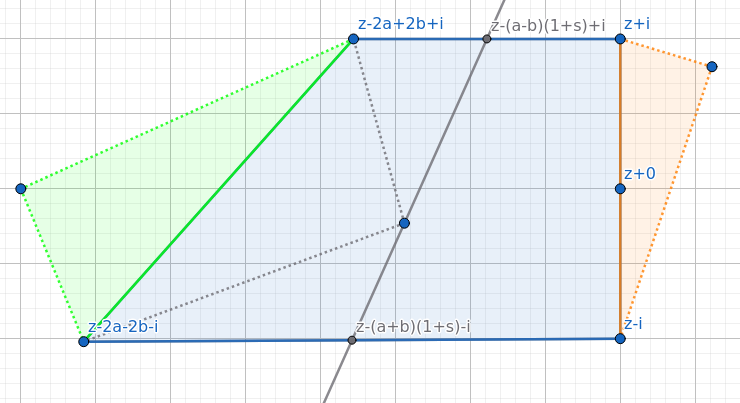
\includegraphics[width=\textwidth]{z45}
Here we have a representation of $z_4$ and $z_5$ parameterised by $s\in[-1,1]$.
We can imagine as $s$ varies, a line connecting $z_4$ and $z_5$ moving leftwards.
It will be useful for us later if we are able to take some value of $\tilde{z}$ and find the value $s$ which would a produce a line going through it.
To simplify things we can recentre by shifting by z $z \leftarrow (z-z=0)$ and let $\tilde{z} \leftarrow \tilde{z}-z$.
This operation can be undone at the end.
Moving the point $0$ along with the line towards the left gives us the point $-\alpha(1+s)$ and we can find the gradient to write the following:
\begin{align}
    (\beta(1+s)+i)t-\alpha(1+s)&=\tilde{z}=:x+iy\\
    \implies t&=y\\
    \beta(1+s)y-\alpha(1+s)&=x\\
    (1+s)(y\beta-\alpha)&=x\\
    s&=\frac{Re(\tilde{z})}{Im(\tilde{z})\beta-\alpha}-1
\end{align}
The usefulness of this formulation is that we are now able to take any arbritary point and find which region it belongs to in the above diagram.
Also given an $s$ for a $z$, we can see that $arg(z_4)-arg(z_5)$ from $s$ onwards is greater than $\pi$ and passes over the branch cut whereas when it takes on values under $s$, we have no issues with branch cuts.
We have the 3 different cases for where the origin can be relative to our value of z which we can go through one by one:

Case 3 $(Re(z)<0)$:
\begin{align}
    arg(z-(\alpha-\beta)(1+s)+i)&>arg(z+i)\\
    arg(z-(\alpha+\beta)(1+s)-i)&<arg(z-i)\\
    \implies arg(z_4)-arg(z_5)&>arg(z+i)-arg(z-i)\\
    &>\pi
\end{align}

Case 4 $(\frac{Re(0-z)}{Im(0-z)\beta-\alpha}>2\implies\frac{Re(z)}{\alpha+Im(z)\beta}>2)$:
\begin{align}
    arg(z-(\alpha-\beta)(1+s)+i)&<arg(z-2(\alpha-\beta)+i)\\
    arg(z-(\alpha+\beta)(1+s)-i)&>arg(z-2(\alpha+\beta)-i)\\
    \implies arg(z_4)-arg(z_5)&<arg(z-2(\alpha-\beta)+i)-arg(z-2(\alpha+\beta)-i)\\
    &<\pi
\end{align}

Case 5 $(s+1:=\frac{Re(z)}{\alpha+Im(z)\beta}\in[0,2])$:
\begin{align}
    s\in[-1,1] &\implies\\
    u\in[0,s+1] &\implies arg(z-(\alpha-\beta)u+i)-arg(z-(\alpha+\beta)u-i)\leq\pi\\
    s+1<u\leq2 &\implies arg(z-(\alpha-\beta)u+i)-arg(z-(\alpha+\beta)u-i)>\pi
\end{align}

From these 3 cases, we can come up with a correction using the following:
\begin{align}
    s &= max\{0, min\{\frac{Re(z)}{\alpha+Im(z)\beta},2\}\}-1\\
    \int_{-1}^1P_k(u)log(\frac{z_4}{z_5})du &=\int_{-1}^sP_k(u)(log(z_4)-log(z_5))du\\
    &+\int_s^1P_k(u)(log(z_4)-log(z_5)-2\pi i)du\\
    &=\int_{-1}^1P_k(u)(log(z_4)-log(z_5))du-2\pi i\int_s^1P_k(u)du\\
    &=\int_{-1}^1P_k(u)(log(z_4)-log(z_5))du-2\pi iC_{k+1}^{(-1/2)}(s)\\
    \int_{-1}^1C_2(s)ds &= -2\pi iC_{k+1}^{(-1/2)}(s)
\end{align}

This gives our final expression for $q_k$:
$$q_k=L_k(\frac{z-i}{\alpha-\beta}-1)-L_k(\frac{z-i}{\alpha+\beta}-1)
+2\delta_{k0}log(\frac{\alpha-\beta}{\alpha+\beta})-2\pi i C_{k+1}^{(-1/2)}(s)$$

\subsubsection*{Case 4: $k=0$}
For this case we are considering how to solve the following:
\begin{align}
    \tilde{s}_{0j} &= \int_{-1}^1\frac{P_j(t)}{\alpha+\beta t}s_0(\tilde{z}_t)dt\\
    &= \int_{-1}^1\frac{P_j(t)}{\alpha+\beta t}log(\frac{\tilde{z}_t+1}{\tilde{z}_t-1})dt
\end{align}
This is difficult to find a closed form solution for, especially for all values of $j$.
We will later be forced into solving this problem with the use of dilogarithms, but we can do it in a way where we only have to do this once rather than for every value of $j$.

We can do the use the fact that we are able to compute all $r_j=s_{0j}$ to help us compute $\tilde{s}_{0j}$.
It is easy to see the relation between $s_{0j}$ and $\tilde{s}_{0j}$ as:
\begin{align}
    j>0 : s_{0j}&=\int_{-1}^1P_j(t)s_0(\tilde{z}_t)dt\\
    &=\int_{-1}^1\frac{(\alpha+\beta t)P_j(t)}{\alpha+\beta t}s_0(\tilde{z}_t)dt\\
    &=\alpha \tilde{s}_{0j} + \beta(j_-\tilde{s}_{0j-1}+j_+\tilde{s}_{0j+1})\\
    j=0 : s_{00}&=\alpha\tilde{s}_{00}+\beta\tilde{s}_{01}
\end{align}
Given a value for $\tilde{s}_{00}$ we are therefore easily able to compute all values of $\tilde{s}_{0j}$ recursively.

\subsubsection*{Case 5: $j=0$}
\begin{align}
    \tilde{s}_{k0} &= \int_{-1}^1\frac{P_k(s)}{\beta(1+s)+i}s_0(\tilde{z}_s)ds\\
    &= \int_{-1}^1\frac{P_k(s)}{\beta(1+s)+i}log(\frac{\tilde{z}_s+1}{\tilde{z}_s-1})ds
\end{align}
Again for the same reasons of not being able to find a closed form solution to this we look for a $q_k$ and use this to find $\tilde{s}_{k0}$.

\begin{align}
    k>0 : q_k &= \int_{-1}^1P_k(s)s_0(\tilde{z}_s)ds\\
    &= \int_{-1}^1\frac{(\beta(1+s)+i)P_k(s)}{\beta(1+s)+i}s_0(\tilde{z}_s)ds\\
    &= (\beta+i)\tilde{s}_{k0} + \beta(k_-\tilde{s}_{k-10}+k_+\tilde{s}_{k+10})\\
    k=0 : q_0 &= (\beta+i)\tilde{s}_{00}+\beta\tilde{s}_{10}
\end{align}

Given a value of $\tilde{s}_{00}$ we are able to compute all values of $\tilde{s}_{k0}$ recursively.
Now the challenge remains to find this $\tilde{s}_{00}$.

\subsubsection*{Case 6: $k,j=0,0$}
We are looking for the following:
\begin{align}
    \tilde{s}_{00}&=\int_{-1}^1\frac{s_0(\tilde{z}_t)}{\alpha+\beta t}dt=\int_{-1}^1\frac{1}{\alpha+\beta t}log(\frac{\tilde{z}_t+1}{\tilde{z}_t-1})dt\\
    &=\int_{-1}^1\frac{1}{\alpha+\beta t}log(\frac{z-it}{z-it-2(\alpha+\beta t)})dt\\
    &=\int_{-1}^1\frac{1}{\alpha+\beta t}log(\frac{z-it}{z-2\alpha-(2\beta+i)t})dt\\
    &=\int_{-1}^1\frac{log(z-it)}{\alpha+\beta t}-\int_{-1}^1\frac{z-2\alpha-(2\beta+i)t}{\alpha+\beta t}dt\\
    &=\frac{1}{\beta}(\int_{-1}^1\frac{log(z-it)}{\alpha/\beta+ t}-\int_{-1}^1\frac{z-2\alpha-(2\beta+i)t}{\alpha/\beta+t}dt)
\end{align}

We need to be able to solve solutions of the following from:
$$\int_{-1}^1\frac{log(z+ct)}{b+t}dt$$
Begin by considering decomposing $log(z+ct)\rightarrow log(\frac{z}{c}+t)+log(c)$.
Rigorously we must show that we do not cross a branch cut for all values of $t$, however, we can notice that the values of $t$ in the decomposed form is along a horizontal line.
We can assume that this interval does not cross over $0$ as our integral needs to be defined.
Because of this we can say that the whole interval either stays or crosses over the cut.
We can therefore add a correction term $(2\pi i)$ depending on $|arg(c)+arg(z/c)|$ and no correction term if this stays under $\pi$.
We can move forward by denoting as $C_3$:
\begin{align}
    \int_{-1}^1\frac{log(z+ct)}{b+t}dt&=\int_{-1}^1\frac{log(z/c+t)}{b+t}+\frac{log(c)}{b+t}dt+C_3\\
    &=\int_{-1}^1\frac{log(z/c+t)}{b+t}dt+log(c)(log(b+1)-log(b-1))+C_3
\end{align}

Now we have an integral in the form $\int_{-1}^1\frac{log(a+t)}{b+t}dt$.
In the case where $a=b$:
\begin{align}
    \int_{-1}^1\frac{log(b+t)}{b+t}dt&=\int_{b-1}^{b+1}\frac{log(t)}{t}dt\\
    u = log(t) \implies &= \int_{log(b-1)}^{log(b+1)}udu\\
    &=(log(b+1)^2-log(b-1)^2)/2
\end{align}
Otherwise if $a\neq b$:
$$\int_{-1}^1\frac{log(a+t)}{b+t}dt=\int_{b-1}^{b+1}\frac{log(a-b+t)}{t}dt$$
We know go about finding correction terms for:$log(a-b+t)\rightarrow log(a-b)+log(1+\frac{t}{a-b})$ as $a-b\in\mathbb{C}$
We have a branch crossing if for some $t\in[-1,1]$:
$$|arg(a+t)-arg(a-b)|>\pi$$
\begin{center}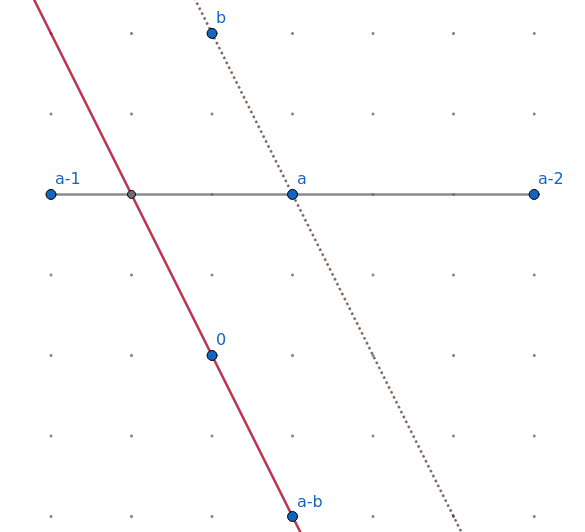
\includegraphics[width=\textwidth/2]{s00}\end{center}
Above we can see an example of $a,b$ values which results in a branch crossing over the positive side.
The red line denotes the angle at which we rotate when dividing by $a-b$.
This means that anything on the left over this line crosses the branch cut whilst anything to the right does not.
Same thing applies in the negative version where the interval of $a$ is in the negative case rotated clockwise over the branch cut.Therefore, we first have to check that a cut exists.
There are many edge cases here which I will not delve into but the rough idea is to check through the args of $a-1,a+1,a-b$ and make comparisons to determine any crossings.
With that we have handled cases where there are either no crossings or where the whole interval has crossed.
It is possible to formulate a way using trig functions to find a value of $t$ where $arg(a+t)=\pi-arg(a-b)$ in the positive case and $arg(a+t)=-\pi+arg(a-b)$ in the negative case.
let $a-b+w=a+t$ so that we have a $w$ which is a representation of the position of our intercept in the $[b-1,b+1]$ interval.
In the case where either the whole interval crosses the branch cut or none of it does we can set it to be the appropriate edge $w\in{b-1,b+1}$. This is useful since we are then able to represent the integral as follows:
\begin{align}
    \int_{-1}^1\frac{log(a+t)}{b+t}dt&=\int_{b-1}^{b+1}\frac{log(a-b+t)}{t}dt=:\int_{b-1}^{b+1}\frac{log(d+t)}{t}dt\\
    &=\int_{b-1}^{w}\frac{\pm2\pi i}{t}dt+\int_{b-1}^{b+1}\frac{log(d)+log(1+t/d)}{t}dt\\
    -u=\frac{t}{d},du=-\frac{dt}{d}:\:&=\pm2\pi ilog(\frac{w}{b-1})+log(a-b)log(\frac{b+1}{b-1})\\
    &+\int_{-\frac{b-1}{a-b}}^{-\frac{b+1}{a-b}}\frac{log(1-u)}{u}du
\end{align}
We can try to solve this using the dilogarithm function:
$$Li_2(z) = -\int_0^z\frac{log(1-u)}{u}du,\:z\in\mathbb{C}$$
We still have to be careful however since there is a branch cut for the dilogarithm function at $(1,\infty)$ at which $Li_2(z+i0^+)-Li_2(z+i0^-) = 2\pi ilog(z),\:z\in(1,\infty)$.
Ignoring edge cases which are less interesting, this can be computed by finding the x-intercept of the interval $[-\frac{b+1}{a-b},-\frac{b-1}{a-b}]$ and checking is this x intercept is part of the branch cut.
We can let $v$ denote the point at which the branch cut is crossed where $v=1$ if there is no crossing through this cut and then we can write:
$$-\int_{-\frac{b-1}{a-b}}^{-\frac{b+1}{a-b}}\frac{log(1-u)}{u}du = Li_2(-\frac{b+1}{a-b})-Li_2(-\frac{b-1}{a-b})\pm2\pi ilog(v)$$
Now that we have all the individual elements we can simply plug everything back in to compute a value for $\tilde{s}_{00}$

\subsubsection{Recovery of $s_{kj}$}
Now we have a situation where we have all values of $\tilde{s}_kj$ but no values for $s_{kj}$.
The basic idea to recover all $s_{kj}$ was by adding consecutive rows together:
$$s_{kj}=\int_{-1}^1P_j(t)s_k(\tilde{z}_t)dt=\int_{-1}^1\frac{\alpha+\beta t}{\alpha+\beta t}P_j(t)s_k(\tilde{z}_t)dt=\alpha\tilde{s}_{kj}+\beta\tilde{s}_{kj+1}$$
\end{document}
